
\begin{figure}
    % generated by Plantuml 1.2022.0
    \definecolor{plantucolor0000}{RGB}{255,255,255}
    \definecolor{plantucolor0001}{RGB}{56,56,56}
    \definecolor{plantucolor0002}{RGB}{248,248,248}
    \definecolor{plantucolor0003}{RGB}{0,0,0}
    \definecolor{plantucolor0004}{RGB}{235,235,235}
    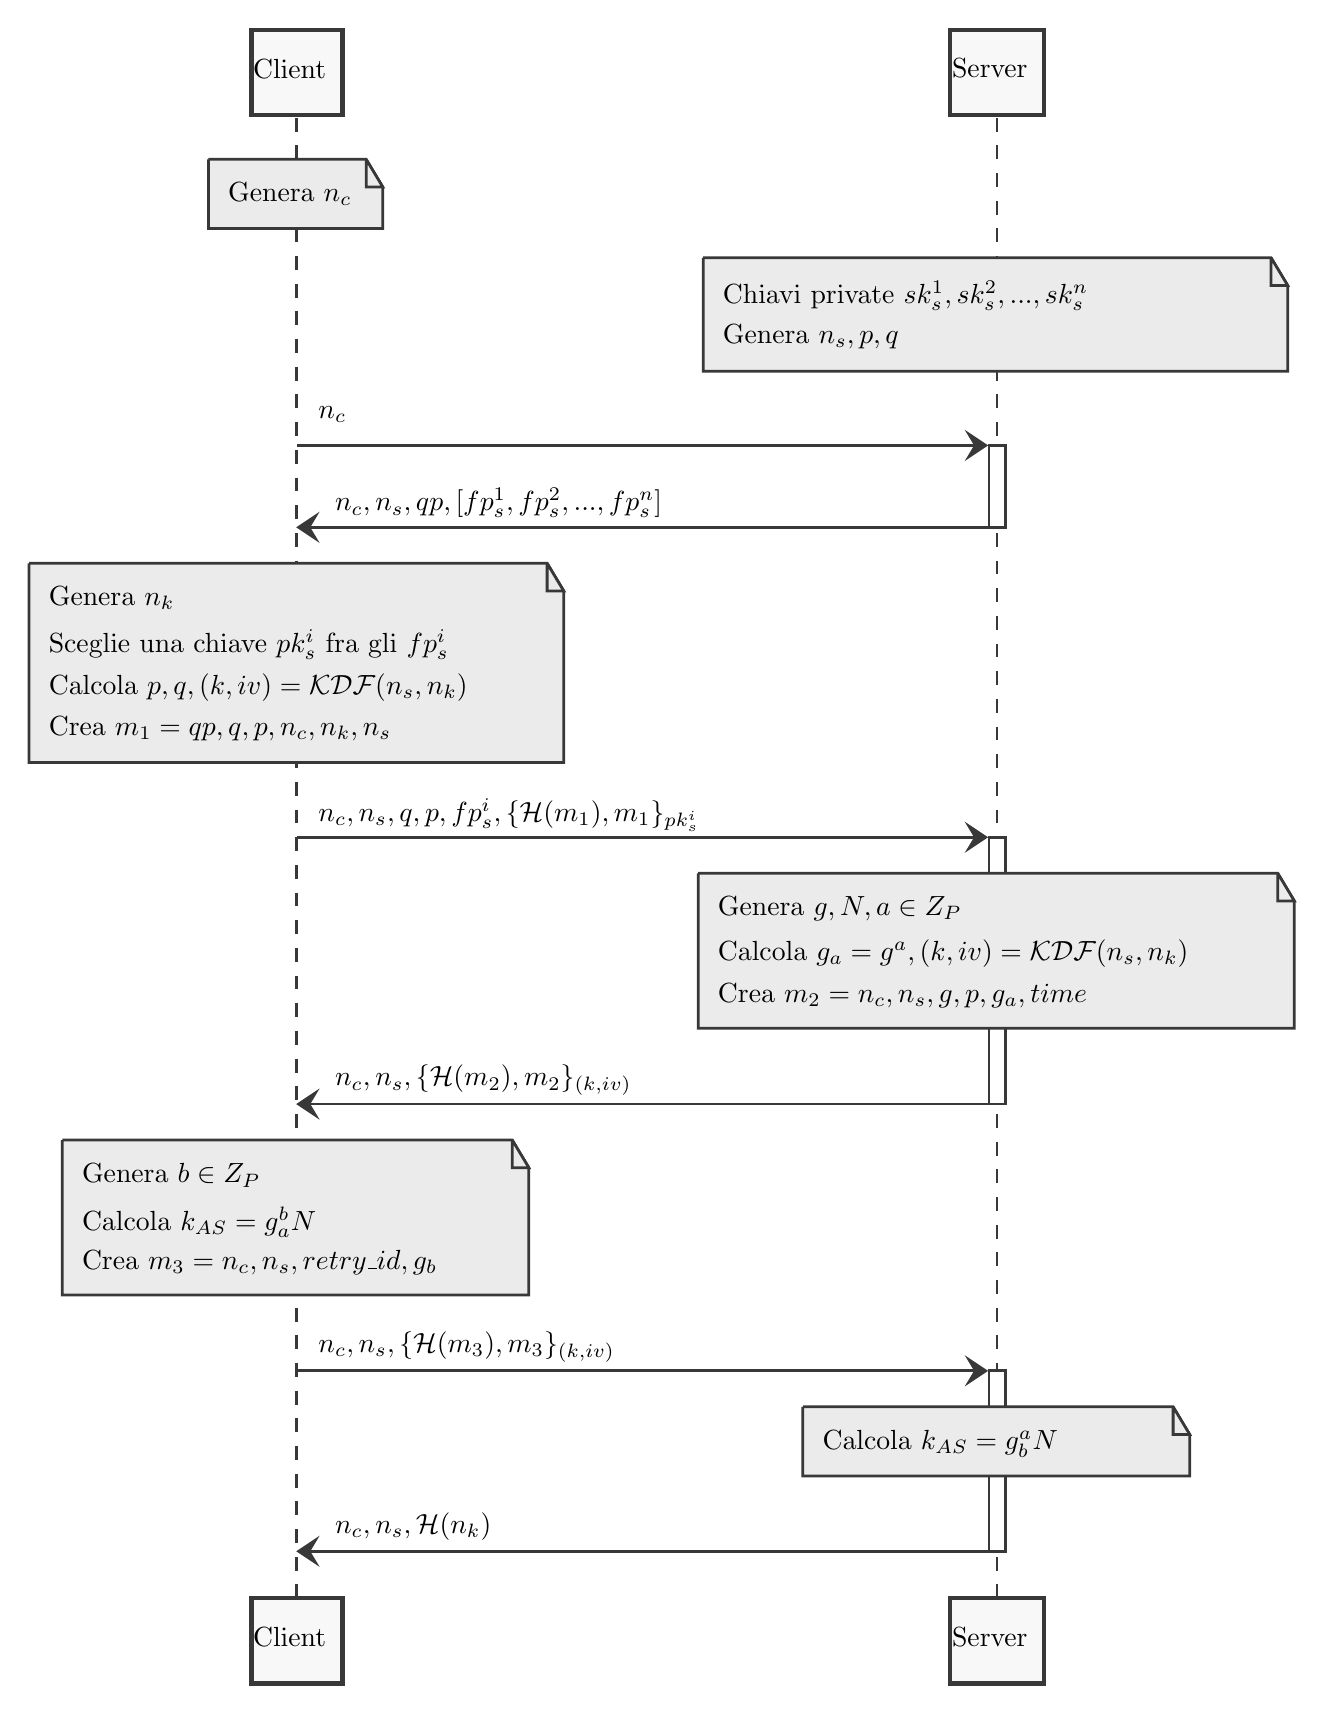
\begin{tikzpicture}[xscale=0.6,yscale=-1
            ,pstyle0/.style={color=plantucolor0001,fill=white,line width=1.0pt}
            ,pstyle1/.style={color=plantucolor0001,line width=1.0pt,dash pattern=on 5.0pt off 5.0pt}
            ,pstyle2/.style={color=plantucolor0001,fill=plantucolor0002,line width=1.5pt}
            ,pstyle3/.style={color=plantucolor0001,fill=plantucolor0004,line width=1.0pt}
            ,pstyle4/.style={color=plantucolor0001,fill=plantucolor0001,line width=1.0pt}
            ,pstyle5/.style={color=plantucolor0001,line width=1.0pt}
        ]
        \draw[pstyle0] (583.0914pt,155.2pt) rectangle (593.0914pt,184.8pt);
        \draw[pstyle0] (583.0914pt,296.8001pt) rectangle (593.0914pt,393.2001pt);
        \draw[pstyle0] (583.0914pt,489.6002pt) rectangle (593.0914pt,554.8002pt);
        \draw[pstyle1] (166pt,36.7999pt) -- (166pt,572.8002pt);
        \draw[pstyle1] (587.8644pt,36.7999pt) -- (587.8644pt,572.8002pt);
        \draw[pstyle2] (139pt,5pt) rectangle (193.8pt,35.7999pt);
        \node at (134pt,12pt)[below right,color=black]{Client};
        \draw[pstyle2] (139pt,571.8002pt) rectangle (193.8pt,602.6001pt);
        \node at (134pt,578.8002pt)[below right,color=black]{Client};
        \draw[pstyle2] (559.8644pt,5pt) rectangle (616.3185pt,35.7999pt);
        \node at (555pt,12pt)[below right,color=black]{Server};
        \draw[pstyle2] (559.8644pt,571.8002pt) rectangle (616.3185pt,602.6001pt);
        \node at (555pt,578.8002pt)[below right,color=black]{Server};
        \draw[pstyle0] (583.0914pt,155.2pt) rectangle (593.0914pt,184.8pt);
        \draw[pstyle0] (583.0914pt,296.8001pt) rectangle (593.0914pt,393.2001pt);
        \draw[pstyle0] (583.0914pt,489.6002pt) rectangle (593.0914pt,554.8002pt);
        \draw[pstyle3] (113pt,51.7999pt) -- (113pt,76.7999pt) -- (218pt,76.7999pt) -- (218pt,61.7999pt) -- (208pt,51.7999pt) -- (113pt,51.7999pt);
        \draw[pstyle3] (208pt,51.7999pt) -- (208pt,61.7999pt) -- (218pt,61.7999pt) -- (208pt,51.7999pt);
        \node at (119pt,56.7999pt)[below right,color=black]{Genera $n_c$};
        \draw[pstyle3] (411pt,87.3999pt) -- (411pt,128.3999pt) -- (763pt,128.3999pt) -- (763pt,97.3999pt) -- (753pt,87.3999pt) -- (411pt,87.3999pt);
        \draw[pstyle3] (753pt,87.3999pt) -- (753pt,97.3999pt) -- (763pt,97.3999pt) -- (753pt,87.3999pt);
        \node at (417pt,92.3999pt)[below right,color=black]{Chiavi private $sk^1_s, sk^2_s, ..., sk^n_s$};
        \node at (417pt,108pt)[below right,color=black]{Genera $n_s, p, q$};
        \draw[pstyle4] (571.0914pt,151.2pt) -- (581.0914pt,155.2pt) -- (571.0914pt,159.2pt) -- (575.0914pt,155.2pt) -- cycle;
        \draw[pstyle5] (166.4pt,155.2pt) -- (577.0914pt,155.2pt);
        \node at (173.4pt,137.6pt)[below right,color=black]{$n_c$};
        \draw[pstyle4] (177.4pt,180.8pt) -- (167.4pt,184.8pt) -- (177.4pt,188.8pt) -- (173.4pt,184.8pt) -- cycle;
        \draw[pstyle5] (171.4pt,184.8pt) -- (587.0914pt,184.8pt);
        \node at (183.4pt,167.2pt)[below right,color=black]{$n_c, n_s, qp, [fp^1_s, fp^2_s, ..., fp^n_s]$};
        \draw[pstyle3] (5pt,197.8pt) -- (5pt,269.8pt) -- (327pt,269.8pt) -- (327pt,207.8pt) -- (317pt,197.8pt) -- (5pt,197.8pt);
        \draw[pstyle3] (317pt,197.8pt) -- (317pt,207.8pt) -- (327pt,207.8pt) -- (317pt,197.8pt);
        \node at (11pt,202.8pt)[below right,color=black]{Genera $n_k$};
        \node at (11pt,218.4pt)[below right,color=black]{Sceglie una chiave $pk^i_s$ fra gli $fp^i_s$};
        \node at (11pt,234pt)[below right,color=black]{Calcola $p, q, (k, iv) = \mathcal{KDF}(n_s, n_k)$};
        \node at (11pt,249.6pt)[below right,color=black]{Crea $m_1 = qp, q, p, n_c, n_k, n_s$};
        \draw[pstyle4] (571.0914pt,292.8001pt) -- (581.0914pt,296.8001pt) -- (571.0914pt,300.8001pt) -- (575.0914pt,296.8001pt) -- cycle;
        \draw[pstyle5] (166.4pt,296.8001pt) -- (577.0914pt,296.8001pt);
        \node at (173.4pt,279.2001pt)[below right,color=black]{$n_c, n_s, q, p, fp^i_s, \{\mathcal{H}(m_1), m_1\}_{pk^i_s}$};
        \draw[pstyle3] (408pt,309.8001pt) -- (408pt,365.8001pt) -- (767pt,365.8001pt) -- (767pt,319.8001pt) -- (757pt,309.8001pt) -- (408pt,309.8001pt);
        \draw[pstyle3] (757pt,309.8001pt) -- (757pt,319.8001pt) -- (767pt,319.8001pt) -- (757pt,309.8001pt);
        \node at (414pt,314.8001pt)[below right,color=black]{Genera $g, N, a \in \mathbb{Z}_P$};
        \node at (414pt,330.4001pt)[below right,color=black]{Calcola $g_a = g^a, (k, iv) = \mathcal{KDF}(n_s, n_k)$};
        \node at (414pt,346.0001pt)[below right,color=black]{Crea $m_2 = n_c, n_s, g, p, g_a, \text{time}$};
        \draw[pstyle4] (177.4pt,389.2001pt) -- (167.4pt,393.2001pt) -- (177.4pt,397.2001pt) -- (173.4pt,393.2001pt) -- cycle;
        \draw[pstyle5] (171.4pt,393.2001pt) -- (587.0914pt,393.2001pt);
        \node at (183.4pt,375.6001pt)[below right,color=black]{$n_c, n_s, \{\mathcal{H}(m_2), m_2\}_{(k, iv)}$};
        \draw[pstyle3] (25pt,406.2001pt) -- (25pt,462.2001pt) -- (306pt,462.2001pt) -- (306pt,416.2001pt) -- (296pt,406.2001pt) -- (25pt,406.2001pt);
        \draw[pstyle3] (296pt,406.2001pt) -- (296pt,416.2001pt) -- (306pt,416.2001pt) -- (296pt,406.2001pt);
        \node at (31pt,411.2001pt)[below right,color=black]{Genera $b \in \mathbb{Z}_P$};
        \node at (31pt,426.8001pt)[below right,color=black]{Calcola $k_{AS} = g^b_a \mod N$};
        \node at (31pt,442.4001pt)[below right,color=black]{Crea $m_3 = n_c, n_s, \text{retry\_id}, g_b$};
        \draw[pstyle4] (571.0914pt,485.6002pt) -- (581.0914pt,489.6002pt) -- (571.0914pt,493.6002pt) -- (575.0914pt,489.6002pt) -- cycle;
        \draw[pstyle5] (166.4pt,489.6002pt) -- (577.0914pt,489.6002pt);
        \node at (173.4pt,472.0002pt)[below right,color=black]{$n_c, n_s, \{\mathcal{H}(m_3), m_3\}_{(k, iv)}$};
        \draw[pstyle3] (471pt,502.6002pt) -- (471pt,527.6002pt) -- (704pt,527.6002pt) -- (704pt,512.6002pt) -- (694pt,502.6002pt) -- (471pt,502.6002pt);
        \draw[pstyle3] (694pt,502.6002pt) -- (694pt,512.6002pt) -- (704pt,512.6002pt) -- (694pt,502.6002pt);
        \node at (477pt,507.6002pt)[below right,color=black]{Calcola $k_{AS} = g^a_b \mod N$};
        \draw[pstyle4] (177.4pt,550.8002pt) -- (167.4pt,554.8002pt) -- (177.4pt,558.8002pt) -- (173.4pt,554.8002pt) -- cycle;
        \draw[pstyle5] (171.4pt,554.8002pt) -- (587.0914pt,554.8002pt);
        \node at (183.4pt,537.2002pt)[below right,color=black]{$n_c, n_s, \mathcal{H}(n_k)$};
    \end{tikzpicture}
    \caption{Diagramma di sequenza dell creazione della chiave di autorizzazione in \gls{mtproto}.
        La funzione hash $\mathcal{H}$ è SHA1.
        $\mathcal{KDF}$ utilizza gli hash di $n_s, n_k$ per generare la chiave temporanea $k$ e il vettore di inizializzazione $iv$}. \label{fig:mtproto-sequence-auth}
\end{figure}
